


\documentclass[english,11pt]{article}
%%%%%%%%%%%%%%%%%%%%%%%%%%%%%%%%%%%%%%%%%%%%%%%%%%%%%%%%%%%%%%%%%%%%%%%%%%%%%%%%%%%%%%%%%%%%%%%%%%%%%%%%%%%%%%%%%%%%%%%%%%%%%%%%%%%%%%%%%%%%%%%%%%%%%%%%%%%%%%%%%%%%%%%%%%%%%%%%%%%%%%%%%%%%%%%%%%%%%%%%%%%%%%%%%%%%%%%%%%%%%%%%%%%%%%%%%%%%%%%%%%%%%%%%%%%%
\usepackage[T1]{fontenc}
\usepackage[latin9]{inputenc}
\usepackage{amsmath}
\usepackage{babel}
\usepackage[symbol]{footmisc}
\usepackage{amsfonts}
\usepackage{makecell}
\usepackage{natbib}
\usepackage{graphicx}

\usepackage{fullpage}
\usepackage{hyperref,url}
\setcounter{MaxMatrixCols}{10}
%TCIDATA{OutputFilter=LATEX.DLL}
%TCIDATA{Version=5.50.0.2960}
%TCIDATA{<META NAME="SaveForMode" CONTENT="1">}
%TCIDATA{BibliographyScheme=Manual}
%TCIDATA{LastRevised=Friday, August 23, 2019 12:15:11}
%TCIDATA{<META NAME="GraphicsSave" CONTENT="32">}
%TCIDATA{Language=American English}


\begin{document}


\begin{center}
\textbf{Economics 600a}

\textbf{Fall 2025}

\textbf{Marek Chadim}\footnote[1]{marek.chadim@yale.edu}

\textbf{Homework Solution}

\end{center}

\bigskip

\section{Overview}

I estimate demand and supply in a stylized model of the market for pay-TV services.
I create my own fake data set
for the industry and do some relatively simple estimation. Then, using the \texttt{pyBLP} package of \citet{conlon2020pyblp}, I estimate the model and perform some merger simulations.

\section{Model}

There are $T$ markets, each with four inside goods $j\in
\{1,2,3,4\}$ and an outside option. Goods 1 and 2 are satellite television
services (e.g., DirecTV and Dish); goods 3 and 4 are wired television
services (e.g., Frontier and Comcast in New Haven).
The conditional indirect utility of consumer $i$ for good $j$ in market $t$
is given by
\begin{align*}
u_{ijt}& =\beta ^{\left( 1\right) }x_{jt}+\beta
_{i}^{(2)}satellite_{jt}+\beta _{i}^{(3)}wired_{jt}+\alpha p_{jt}+\xi
_{jt}+\epsilon _{ijt}\text{ \qquad }j>0 \\
u_{i0t}& =\epsilon _{i0t},
\end{align*}%
where $x_{jt}$ is a measure of good $j$'s quality, $p_{jt}$ is its price, $%
satellite_{jt}$ is an indicator equal to 1 for the two satellite services,
and $wired_{jt}$ is an indicator equal to 1 for the two wired services. The
remaining notation is as usual in the class notes, including the i.i.d.
type-1 extreme value $\epsilon _{ijt}$.  Each consumer purchases the good giving them the highest conditional indirect utility.

Goods are produced by single-product firms. Firm $j$'s (log) marginal
cost in market $t$ is 
\begin{equation*}
\ln mc_{jt}=\gamma ^{0}+\text{w}_{jt}\gamma ^{1}+\omega _{jt}/8,
\end{equation*}%
where w$_{jt}$ is an observed cost shifter. Firms compete by simultaneously choosing prices in each market under complete information. Firm $j$ has profit
\begin{equation*}
\pi _{jt}=\max_{p_{jt}}M_{t}(p_{jt}-mc_{jt})s_{jt}(p_{t}).
\end{equation*}

\section{Generate Fake Data}

Generate a data set from the model above. Start with%
\begin{eqnarray*}
\beta ^{(1)} &=&1\text{, }\beta _{i}^{\left( k\right) }\sim \text{iid }%
N\left( 4,1\right) \text{ for }k=2,3 \\
\alpha  &=&-2 \\
\gamma ^{(0)} &=&1/2\text{, }\gamma ^{(1)}=1/4.
\end{eqnarray*}

\begin{enumerate}
\item Draw the exogenous product characteristic $x_{jt}$ for $T=600$
geographically defined markets (e.g., cities). Assume each $x_{jt}$ is equal
to the absolute value of an iid standard normal draw, as is each w$_{jt}$.
Simulate demand and cost unobservables as well, specifying
\begin{equation*}
\left(
\begin{array}{c}
\xi _{jt} \\
\omega _{jt}%
\end{array}%
\right) \sim N\left( \left(
\begin{array}{c}
0 \\
0%
\end{array}%
\right) ,\left(
\begin{array}{cc}
1 & 0.25 \\
0.25 & 1%
\end{array}%
\right) \right) \text{ iid across }j,t.
\end{equation*}


\begin{verbatim}
np.random.seed(1995)
# Model parameters
T, J = 600, 4
alpha, beta1 = -2, 1
beta2, beta3 = 4, 4  
sigma_satellite, sigma_wired = 1, 1
gamma0, gamma1 = 0.5, 0.25
# Product data structure
data = [
    {'market_ids': t, 'firm_ids': j+1, 'product_ids': j} 
    for t in range(T) 
    for j in range(J)
]
product_data = pd.DataFrame(data)
# Exogenous variables: x_jt and w_jt as absolute values of iid standard normal draws
product_data['x'] = np.abs(
    np.random.normal(0, 1, len(product_data))
)
product_data['w'] = np.abs(
    np.random.normal(0, 1, len(product_data))
)
# Indicators
product_data['satellite'] = (
    product_data['firm_ids'].isin([1, 2]).astype(int)
)
product_data['wired'] = (
    product_data['firm_ids'].isin([3, 4]).astype(int)
)
# Unobservables: xi_jt and omega_jt with covariance matrix [[1, 0.25], [0.25, 1]]
cov_matrix = np.array([[1, 0.25], [0.25, 1]])
A = np.linalg.cholesky(cov_matrix)
z = np.random.normal(0, 1, (len(product_data), 2))
unobs = z @ A.T
product_data['xi'] = unobs[:, 0]  # demand unobservable
product_data['omega'] = unobs[:, 1]  # cost unobservable
\end{verbatim}

\item Solve for the equilibrium prices for each good in each market.

\begin{enumerate}
\item Start by writing a procedure to approximate the derivatives of market
shares with respect to prices (taking prices, shares, $x$, and demand
parameters as inputs). The key steps are:
\begin{enumerate}
\item For each $(j,t)$, write the choice probability $s_{jt}$ as a weighted
average (integral) of the (multinomial logit) choice probabilities
conditional on the value of each consumer's random coefficients; 

\textbf{Answer:}

From the utility specification, we can write:
\begin{equation*}
u_{ijt} = \delta_{jt} + \nu_{ijt}
\end{equation*}
where the mean utility is
\begin{equation*}
\delta_{jt} = \beta^{(1)}x_{jt} + \alpha p_{jt} + \xi_{jt}
\end{equation*}
and the individual deviation is
\begin{equation*}
\nu_{ijt} = \beta_i^{(2)}satellite_{jt} + \beta_i^{(3)}wired_{jt} + \epsilon_{ijt}.
\end{equation*}

Given the random coefficients $\beta_i = (\beta_i^{(2)}, \beta_i^{(3)})$ and the Type-1 extreme value distribution of $\epsilon_{ijt}$, the conditional choice probability follows the multinomial logit form \citep{berry1995automobile}:
\begin{equation*}
s_{jt}|\beta_i = \frac{\exp(\delta_{jt} + \beta_i^{(2)}satellite_{jt} + \beta_i^{(3)}wired_{jt})}{1 + \sum_{k=1}^4 \exp(\delta_{kt} + \beta_i^{(2)}satellite_{kt} + \beta_i^{(3)}wired_{kt})}.
\end{equation*}

The unconditional market share is the integral over the distribution of random coefficients:
\begin{equation*}
s_{jt} = \int \frac{\exp(\delta_{jt} + \beta_i^{(2)}satellite_{jt} + \beta_i^{(3)}wired_{jt})}{1 + \sum_{k=1}^4 \exp(\delta_{kt} + \beta_i^{(2)}satellite_{kt} + \beta_i^{(3)}wired_{kt})} f(\beta_i^{(2)}, \beta_i^{(3)}) \, d\beta_i^{(2)} d\beta_i^{(3)}
\end{equation*}
where $f(\cdot)$ is the joint density of $(\beta_i^{(2)}, \beta_i^{(3)})$, with each $\sim N(4,1)$ independently.


\item Anticipating differentiation under the integral sign, derive the
analytical expression for the derivative of the \textit{integrand} with
respect to each $p_{kt}$; 

\textbf{Answer:}

Let the integrand be denoted as:
\begin{equation*}
I_{jt}(\beta_i) = \frac{\exp(\delta_{jt} + \beta_i^{(2)}satellite_{jt} + \beta_i^{(3)}wired_{jt})}{1 + \sum_{\ell=1}^4 \exp(\delta_{\ell t} + \beta_i^{(2)}satellite_{\ell t} + \beta_i^{(3)}wired_{\ell t})}.
\end{equation*}

Since $\delta_{kt} = \beta^{(1)}x_{kt} + \alpha p_{kt} + \xi_{kt}$, we have $\frac{\partial \delta_{kt}}{\partial p_{kt}} = \alpha$.

For $k = j$ (own-price derivative):
\begin{align*}
\frac{\partial I_{jt}}{\partial p_{jt}} &= \alpha \cdot I_{jt}(\beta_i) \cdot (1 - I_{jt}(\beta_i))
\end{align*}

For $k \neq j$ (cross-price derivative):
\begin{align*}
\frac{\partial I_{jt}}{\partial p_{kt}} &= -\alpha \cdot I_{jt}(\beta_i) \cdot I_{kt}(\beta_i)
\end{align*}

where $I_{kt}(\beta_i)$ is the conditional choice probability for good $k$:
\begin{equation*}
I_{kt}(\beta_i) = \frac{\exp(\delta_{kt} + \beta_i^{(2)}satellite_{kt} + \beta_i^{(3)}wired_{kt})}{1 + \sum_{\ell=1}^4 \exp(\delta_{\ell t} + \beta_i^{(2)}satellite_{\ell t} + \beta_i^{(3)}wired_{\ell t})}.
\end{equation*}

These are the standard multinomial logit derivative formulas, conditional on $\beta_i$.


\item Use the expression you obtained in (2) and simulation draws of the
random coefficients to approximate the integral that corresponds to $%
\partial s_{jt}/\partial p_{kt}$ for each $j$ and $k$ (i.e., replace
the integral with the mean over the values at each simulation draw). Recall the advice in the lecture regarding \textquotedblleft
jittering.\textquotedblright\ \newline

\begin{verbatim}
def market_shares_and_derivatives(prices, market_data, nu_draws):
    J = len(market_data)
    x = market_data['x'].values
    xi = market_data['xi'].values
    sat = market_data['satellite'].values
    wired = market_data['wired'].values
    
    # Compute utilities once
    utilities = (
        beta1 * x + xi + 
        nu_draws[:, 0:1] * sat + 
        nu_draws[:, 1:2] * wired + 
        alpha * prices
    )
    utilities = np.column_stack([utilities, np.zeros(nu_draws.shape[0])])
    exp_u = np.exp(utilities - np.max(utilities, axis=1, keepdims=True))
    choice_probs = exp_u / exp_u.sum(axis=1, keepdims=True)
    inside_shares_draws = choice_probs[:, :J]
    
    # Shares: average over draws
    shares = np.mean(inside_shares_draws, axis=0)
    
    # Derivatives: compute analytically from choice probabilities
    derivatives = np.zeros((J, J))
    for j in range(J):
        for k in range(J):
            indicator = float(j == k)
            deriv_draws = (
                alpha * inside_shares_draws[:, j] * 
                (indicator - inside_shares_draws[:, k])
            )
            derivatives[j, k] = np.mean(deriv_draws)
    
    return shares, derivatives, inside_shares_draws
\end{verbatim}

\newline

I do not want to take new simulation draws of the random
coefficients each time I call this procedure. This is because,  if I did so, the attempt
to solve for equilibrium prices (below) may never converge due to \textquotedblleft
jittering\textquotedblright\ across iterations. So I take simulation draws only once, outside the procedure I wrote here. 

\begin{verbatim}
all_nu_draws = [np.random.multivariate_normal([beta2, beta3], 
np.diag([sigma_satellite, sigma_wired]), size=10000) for _ in range(T)]
\end{verbatim}


    \item Experiment to see how many simulation draws you need to get precise
    approximations and check this again at the equilibrium shares and prices you
    obtain below. 
    
    \textbf{Answer:}
    
I test convergence by computing derivatives multiple times with different random draws and measuring the standard deviation across repetitions:

\begin{verbatim}
def test_convergence(prices, market_data, nu_draws_full, 
                     draw_counts, n_reps=100):
    stds = []
    n_available = len(nu_draws_full)
    for n_draws in draw_counts:
        deriv_list = []
        for rep in range(n_reps):
            # Randomly sample n_draws from pre-drawn samples
            indices = np.random.choice(n_available, size=n_draws, 
                                       replace=False)
            nu_draws = nu_draws_full[indices]
            _, derivs, _ = market_shares_and_derivatives(
                prices, market_data, nu_draws
            )
            deriv_list.append(derivs)
        stds.append(np.std(deriv_list, axis=0).mean())
    return np.array(stds)
# Test at initial prices (p = MC) for market 0
product_data['mc'] = np.exp(
    gamma0 + gamma1 * product_data['w'] + product_data['omega'] / 8
)
market_0 = product_data[product_data['market_ids'] == 0]
prices_init = market_0['mc'].values
draw_counts = [50, 100, 200, 500, 1000, 2000, 5000]
stds = test_convergence(prices_init, market_0, all_nu_draws[0], draw_counts)
\end{verbatim}

\textbf{Convergence Results at Initial Prices:}

\begin{center}
\begin{tabular}{r|c|r}
Draws & Mean Std Dev & Rel. Change \\
\hline
50    & 0.0080  & --    \\
100   & 0.0054  & 33.2\% \\
200   & 0.0037  & 30.6\% \\
500   & 0.0025  & 32.0\% \\
1000  & 0.0017  & 34.8\% \\
2000  & 0.0011  & 35.1\% \\
5000  & 0.0005  & 51.0\% \\
\end{tabular}
\end{center}

The standard deviation decreases monotonically with the number of simulation draws. With 5,000 draws, the standard deviation is 0.005, which arguably provides a sufficiently precise approximation.

\end{enumerate}


\item The FOC for firm $j$'s profit maximization problem in market $t$ is
\begin{align}
(p_{jt}-mc_{jt})\frac{\partial s_{jt}(p_{t})}{\partial p_{jt}}+s_{jt}& =0
\notag \\
\implies p_{jt}-mc_{jt}& =-\left( \frac{\partial s_{jt}(p_{t})}{\partial
p_{jt}}\right) ^{-1}s_{jt}  \label{FOC}
\end{align}

\item Substituting in your approximation of each $\left( \frac{\partial
s_{jt}(p_{t})}{\partial p_{jt}}\right) $, solve the system of equations (\ref%
{FOC}) ($J\,$equations per market) for the equilibrium prices in each market.

\begin{enumerate}
\item To do this you will need to solve a system of $J \times J$ nonlinear equations. Make sure to check the exit flag for each market to make sure you have a solution.


\begin{verbatim}
def solve_prices_direct(market_data, mc_market, nu_draws):
    J = len(market_data)
    def foc_residual(prices):
        # Compute shares and derivatives at current prices
        shares, derivatives, _ = market_shares_and_derivatives(
            prices, market_data, nu_draws
            )
        # Inversion of derivative matrix
        invD = np.linalg.inv(derivatives)
        # FOC residuals:
        residuals = prices - mc_market + invD @ shares
        return residuals
    # Initial guess: marginal costs
    p0 = mc_market.copy()
    # Solve using root finder (hybr method)
    sol = opt.root(foc_residual, p0, method='hybr', tol=1e-8)
    prices_sol = sol.x
    success = sol.success
    return prices_sol, success
# Solve using direct method
equilibrium_prices_direct = []
success_flags_direct = []
for t in range(T):
    market_data = product_data[product_data['market_ids'] == t]
    mc_market = market_data['mc'].values
    nu_draws = all_nu_draws[t]
    prices_direct, success = solve_prices_direct(
        market_data, mc_market, nu_draws
        )
    equilibrium_prices_direct.append(prices_direct)
    success_flags_direct.append(success)
equilibrium_prices_direct = np.array(equilibrium_prices_direct)
success_count = sum(success_flags_direct)
\end{verbatim}

\textbf{Results:} Successfully solved 600/600 markets. 


\item Do this again using the algorithm of Morrow and
Skerlos (2011), discussed in section 3.6 of \citet{conlon2020pyblp} (and
in the \texttt{pyBLP} \textquotedblleft problem simulation tutorial\textquotedblright
). Use the numerical integration approach you used in step (a) to approximate the
terms defined in equation (25) of \citet{conlon2020pyblp}. If you get different
results using this method, resolve this discrepancy either by correcting
your code or explaining why your preferred method is the one to be trusted.
\end{enumerate}

\begin{verbatim}
def solve_prices_morrow_skerlos(market_data,
mc_market, nu_draws, max_iter=100, tol=1e-6):
    prices = mc_market.copy()
    for iteration in range(max_iter):
        shares, derivatives, inside_shares_draws = 
        market_shares_and_derivatives(prices, market_data, nu_draws)
        Lambda = np.diag(alpha * shares)
        Gamma = 
        alpha * (inside_shares_draws.T @ inside_shares_draws) / nu_draws.shape[0]
        diff = prices - mc_market
        zeta = np.linalg.solve(Lambda, Gamma.T @ diff - shares)
        prices_new = mc_market + zeta
        foc_residual = Lambda @ (prices - mc_market - zeta)
        if np.max(np.abs(foc_residual)) < tol:
            break
        prices = 0.5 * prices + 0.5 * prices_new
    return prices, iteration + 1
    
# Solve using Morrow-Skerlos method
equilibrium_prices_ms = []
iterations_ms = []
for t in range(T):
    market_data = product_data[product_data['market_ids'] == t]
    mc_market = market_data['mc'].values
    nu_draws = all_nu_draws[t]
    prices_ms, iters = solve_prices_morrow_skerlos(market_data, mc_market, nu_draws)
    equilibrium_prices_ms.append(prices_ms)
    iterations_ms.append(iters)
equilibrium_prices_ms = np.array(equilibrium_prices_ms)

# Compare direct vs Morrow-Skerlos 
    price_diff = np.abs(np.array(equilibrium_prices_direct) - equilibrium_prices_ms)
    
# Use Morrow-Skerlos prices
product_data['prices'] = equilibrium_prices_ms.flatten()
\end{verbatim}


\textbf{Results:} Successfully solved 600/600 markets. 

The Morrow-Skerlos method produces virtually identical results to the direct method (differences of order $10^{-6}$).


\begin{verbatim}
    # Compare derivative convergence at initial vs equilibrium prices
    prices_equilibrium = market_0['prices'].values
    initial_stds = stds 
    n_available = len(all_nu_draws[0])
    n_reps = 100
    eq_stds = []
    for n_draws in draw_counts:
        deriv_list = []
        for _ in range(n_reps):
            indices = np.random.choice(n_available, size=n_draws, replace=False)
            nu_draws = all_nu_draws[0][indices]
            _, derivatives, _ = market_shares_and_derivatives(
                prices_equilibrium, market_0, nu_draws)
            deriv_list.append(derivatives)
        eq_stds.append(np.std(deriv_list, axis=0).mean())
    eq_stds = np.array(eq_stds)
    ratios = eq_stds / initial_stds
    avg_ratio = np.mean(ratios)
\end{verbatim}



 \textbf{Results:} The derivative approximation via Monte Carlo integration is more stable at equilibrium prices compared to initial prices (marginal costs), as the ratio remains consistently around 0.68 across all draw counts.

\begin{center}
\begin{tabular}{r|c|c|c}
Draws & Initial Std Dev & Equilibrium Std Dev & Ratio (Eq/Init) \\
\hline
50    & 0.0080 & 0.0053 & 0.66 \\
100   & 0.0054 & 0.0036 & 0.68 \\
200   & 0.0037 & 0.0027 & 0.71 \\
500   & 0.0025 & 0.0017 & 0.68 \\
1000  & 0.0017 & 0.0011 & 0.69 \\
2000  & 0.0011 & 0.0007 & 0.68 \\
5000  & 0.0005 & 0.0004 & 0.67 \\
\end{tabular}
\end{center}
\end{enumerate}
\item Calculate \textquotedblleft observed\textquotedblright\ shares for
your fake data set using your parameters, your draws of $x,$w$,\beta
_{i},\omega ,\xi $, and your equilibrium prices.
\begin{verbatim}
observed_shares = []
for t in range(T):
    market_data = product_data[product_data['market_ids'] == t]
    prices_market = market_data['prices'].values
    # Use pre-drawn simulation draws for this market
    shares_market, _, _ = market_shares_and_derivatives(
        prices_market, market_data, all_nu_draws[t])
    observed_shares.extend(shares_market)
product_data['shares'] = observed_shares
\end{verbatim}
\textbf{Results:} Share range: 0.000 to 0.725, mean: 0.136 (std: 0.122). Market share sums average 0.543 (min: 0.303, max: 0.746), implying outside shares average 0.457. Average satellite product share: 0.135; average wired product share: 0.136.


\item

Below you'll be using x and w as instruments in the demand estimation. Check whether these appear to be good instruments in your fake data using some regressions of prices and market shares on the exogenous variables (or some function of them; see the related discussion in the coding tips). If you believe the instruments are not providing enough variation, modify the parameter choices above until you are satisfied. Report your final choice of parameters and the results you rely on to conclude that the instruments seem good enough.
\end{enumerate}
\begin{verbatim}
# Create instruments: quadratics, interactions, competitor sums, within-nest
product_data['x**2'] = product_data['x'] ** 2
product_data['w**2'] = product_data['w'] ** 2
product_data['x*w'] = product_data['x'] * product_data['w']
product_data['sum_x_competitors'] = 
product_data.groupby('market_ids')['x'].transform('sum') - product_data['x']
product_data['sum_w_competitors'] = 
product_data.groupby('market_ids')['w'].transform('sum') - product_data['w']
product_data['x_other_in_nest'] = 
product_data.groupby(['market_ids','satellite'])['x'].transform('sum')-product_data['x']
product_data['w_other_in_nest'] = 
product_data.groupby(['market_ids','satellite'])['w'].transform('sum')-product_data['w']

Z = product_data[['satellite', 'wired', 'x', 'w', 'x**2', 'w**2', 'x*w', 
                   'sum_x_competitors', 'sum_w_competitors', 
                   'x_other_in_nest', 'w_other_in_nest']]

# Test instrument validity
price_model = sm.OLS(product_data['prices'], Z).fit()
share_model = sm.OLS(product_data['shares'], Z).fit()
xi_model = sm.OLS(product_data['xi'], Z).fit()
omega_model = sm.OLS(product_data['omega'], Z).fit()

# Joint F-tests for excluded instruments
excluded_vars = ['w', 'x**2', 'w**2', 'x*w', 'sum_x_competitors', 
                 'sum_w_competitors', 'x_other_in_nest', 'w_other_in_nest']
hypothesis = ', '.join([f'{var}=0' for var in excluded_vars])
price_f_test = price_model.f_test(hypothesis)
share_f_test = share_model.f_test(hypothesis)
xi_f_test = xi_model.f_test(hypothesis)
omega_f_test = omega_model.f_test(hypothesis)
\end{verbatim}


\textbf{Results:} The parameters $\alpha = -2$, $\beta^{(1)} = 1$, $\beta_i^{(2)} \sim N(4, 1^2)$, $\beta_i^{(3)} \sim N(4, 1^2)$, $\gamma^{(0)} = 0.5$, $\gamma^{(1)} = 0.25$ were retained as final. Excluded demand instruments (w, x$^2$, w$^2$, x*w, competitor sums, within-nest variables) are relevant based on prices regression R$^2$=0.511, F=301.04 (p$<$0.001) and shares regression R$^2$=0.364, F=91.06 (p$<$0.001). They are also uncorrelated with structural errors: $\xi$ F=0.63 (p=0.75) and $\omega$ F=0.58 (p=0.80).


\section{Estimate Some Mis-specified Models}

\begin{enumerate}
\item[5.] Estimate the multinomial logit model of demand by OLS
(ignoring the endogeneity of prices). \begin{verbatim}
# Compute logit delta: ln(s_jt / s_0t)
product_data['logit_delta'] =
np.log(product_data['shares'] / product_data['outside_share'])

# OLS: beta_hat = (X^T X)^(-1) X^T y
y = product_data['logit_delta'].values
X = product_data[['prices', 'x', 'satellite', 'wired']].values
beta_hat = np.linalg.inv(X.T @ X) @ X.T @ y

# HC0 robust standard errors
residuals = y - X @ beta_hat
V = X.T @ np.diag(residuals**2) @ X
cov_matrix_ols = np.linalg.inv(X.T @ X) @ V @ np.linalg.inv(X.T @ X)
se_ols = np.sqrt(np.diag(cov_matrix_ols))
\end{verbatim}

\textbf{Results:}

OLS estimates for $\ln(s_{jt}/s_{0t}) = \alpha p_{jt} + \beta^{(1)} x_{jt} + \beta^{(2)} satellite_{jt} + \beta^{(3)} wired_{jt}$ (no intercept):

\begin{center}
\begin{tabular}{lrrrr}
\hline
Parameter & Estimate & Std. Error & t-stat & p-value \\
\hline
$\alpha$ (prices) & $-1.246$ & $0.051$ & $-24.41$ & $0.000$ \\
$\beta^{(1)}$ (x) & $0.854$ & $0.032$ & $26.36$ & $0.000$ \\
$\beta^{(2)}$ (satellite) & $1.757$ & $0.165$ & $10.67$ & $0.000$ \\
$\beta^{(3)}$ (wired) & $1.790$ & $0.164$ & $10.90$ & $0.000$ \\
\hline
\end{tabular}
\end{center}
\item[6.] Re-estimate the multinomial logit model of demand by two-stage
least squares, instrumenting for prices with the exogenous demand shifters $%
x $ and excluded cost shifters w. Discuss the predictive value of the instruments in the first stage, and how the second-stage results differ from those
obtained by OLS. \begin{verbatim}
# First stage: regress prices on instruments
Z = product_data[['satellite', 'wired', 'x', 'w', 'x**2', 'w**2', 
                   'x*w', 'sum_x_competitors', 'sum_w_competitors']].values
sigma_hat = np.linalg.inv(Z.T @ Z) @ Z.T @ product_data['prices'].values
prices_hat = Z @ sigma_hat
resid_fs = product_data['prices'].values - prices_hat
SST = np.sum((product_data['prices'].values - product_data['prices'].mean())**2)
SSR = np.sum(resid_fs**2)
R2_first = 1 - SSR/SST
# Second stage
X_hat = np.column_stack([prices_hat, product_data['x'].values,
         product_data['satellite'].values, product_data['wired'].values])
beta_hat_iv = np.linalg.inv(X_hat.T @ X_hat) @ X_hat.T @ y
# HC0 robust SE for 2SLS
X = np.column_stack([product_data['prices'].values, product_data['x'].values,
     product_data['satellite'].values, product_data['wired'].values])
resid_iv = y - X @ beta_hat_iv
P_Z = Z @ np.linalg.inv(Z.T @ Z) @ Z.T
Omega = np.diag(resid_iv**2)
XPZ = X.T @ P_Z
cov_iv = np.linalg.inv(XPZ @ X) @ XPZ @ Omega @ P_Z @ X @ np.linalg.inv(XPZ @ X)
se_iv = np.sqrt(np.diag(cov_iv))
\end{verbatim}


\textbf{Results:} First stage R$^2$ = 0.507 confirms strong instruments.

Second stage 2SLS estimates:

\begin{center}
\begin{tabular}{lrrrr}
\hline
Parameter & Estimate & Std. Error & t-stat & p-value \\
\hline
$\alpha$ (prices) & $-1.938$ & $0.064$ & $-30.51$ & $0.000$ \\
$\beta^{(1)}$ (x) & $0.923$ & $0.035$ & $26.15$ & $0.000$ \\
$\beta^{(2)}$ (satellite) & $3.993$ & $0.208$ & $19.21$ & $0.000$ \\
$\beta^{(3)}$ (wired) & $4.034$ & $0.209$ & $19.34$ & $0.000$ \\
\hline
\end{tabular}
\end{center}

2SLS recovers parameters close to the truth ($\alpha = -2$, $\beta^{(1)} = 1$, $\beta^{(2)}, \beta^{(3)} \sim N(4,1)$). OLS severely underestimates because equilibrium pricing implies each $p_{jt}$ depends on all demand shocks $\xi_t = (\xi_{1t}, \ldots, \xi_{Jt})$ and all cost shocks $\omega_t = (\omega_{1t}, \ldots, \omega_{Jt})$---both through first-order conditions and strategic complementarity \citep{berry2021foundations}. The covariance $\text{Cov}(\xi_{jt}, \omega_{jt}) = 0.25$ creates positive correlation between $\xi_{jt}$ and $p_{jt}$, biasing $\hat{\alpha}_{\text{OLS}}$ toward zero. Cost shifters $w_{jt}$ serve as valid instruments because they shift equilibrium prices (relevance) while satisfying $E[\xi_{jt} | x_t, w_t] = 0$ (exogeneity), breaking the endogeneity between prices and demand unobservables.


\item[7.] Now estimate a nested logit model by two-stage least squares,
treating \textquotedblleft satellite\textquotedblright\ and
\textquotedblleft wired\textquotedblright\ as the two nests for the inside
goods. Allow a different nesting parameter for each nest.

\begin{verbatim}
# Within-group shares for nesting
product_data["group_share"] = product_data.groupby(
    ["market_ids", "satellite"])["shares"].transform("sum")
product_data["ln_within_share"] = np.log(
    product_data["shares"] / product_data["group_share"])

# Nest-specific within-group share variables
product_data["ln_within_share_sat"] = (
    product_data["ln_within_share"] * product_data["satellite"])
product_data["ln_within_share_wired"] = (
    product_data["ln_within_share"] * product_data["wired"])

# First stage: instrument for prices, ln_within_share_sat, ln_within_share_wired
Z = product_data[['x', 'satellite', 'wired', 'w', 'x**2', 'w**2', 'x*w',
                   'sum_x_competitors', 'sum_w_competitors', 
                   'x_other_in_nest', 'w_other_in_nest']].values
endog_vars = ['prices', 'ln_within_share_sat', 'ln_within_share_wired']
endog_hat = np.zeros((len(product_data), 3))
for i, var in enumerate(endog_vars):
    sigma = np.linalg.inv(Z.T @ Z) @ Z.T @ product_data[var].values
    endog_hat[:, i] = Z @ sigma

# Second stage
X_hat = np.column_stack([endog_hat[:, 0], product_data['x'].values,
         product_data['satellite'].values, product_data['wired'].values,
         endog_hat[:, 1], endog_hat[:, 2]])
beta_hat_nl = np.linalg.inv(X_hat.T @ X_hat) @ X_hat.T @ y

# HC0 robust SE for 2SLS
X = np.column_stack([product_data['prices'].values, product_data['x'].values,
     product_data['satellite'].values, product_data['wired'].values,
     product_data['ln_within_share_sat'].values, 
     product_data['ln_within_share_wired'].values])
resid = y - X @ beta_hat_nl
P_Z = Z @ np.linalg.inv(Z.T @ Z) @ Z.T
XPZ = X.T @ P_Z
cov_nl = 
np.linalg.inv(XPZ @ X) @ XPZ @ np.diag(resid**2) @ P_Z @ X @ np.linalg.inv(XPZ @ X)
se_nl = np.sqrt(np.diag(cov_nl))
\end{verbatim}

\textbf{Results:} Nested logit 2SLS estimates (prices, within-group shares instrumented):

\begin{center}
\begin{tabular}{lrrrr}
\hline
Parameter & Estimate & Std. Error & t-stat & p-value \\
\hline
$\alpha$ (prices) & $-1.605$ & $0.097$ & $-16.51$ & $0.000$ \\
$\beta^{(1)}$ (x) & $0.802$ & $0.041$ & $19.53$ & $0.000$ \\
$\beta^{(2)}$ (satellite) & $3.106$ & $0.603$ & $5.15$ & $0.000$ \\
$\beta^{(3)}$ (wired) & $3.348$ & $0.484$ & $6.92$ & $0.000$ \\
$\rho_{sat}$ (ln\_within\_sat) & $0.115$ & $0.449$ & $0.26$ & $0.797$ \\
$\rho_{wired}$ (ln\_within\_wired) & $0.312$ & $0.465$ & $0.67$ & $0.502$ \\
\hline
\end{tabular}
\end{center}

The nesting parameters ($\rho_{sat} = 0.115$, $\rho_{wired} = 0.312$) are not significantly different from zero and lie far from the theoretical bounds $\rho \in (0,1)$ needed for well-defined choice probabilities. This failure arises because the nested logit imposes correlation through $Cov(\epsilon_{ijt}, \epsilon_{ikt} | i, t) = (1-\rho^2)\pi^2/6$ for products $j,k$ in the same nest, effectively modeling substitution patterns through the error structure. The true DGP instead generates substitution via random coefficients $\beta_i^{(2)}, \beta_i^{(3)} \sim N(4,1)$ on satellite/wired indicators, creating heterogeneous valuations $u_{ijt} = -\alpha p_{jt} + \beta_i^{(2)} \cdot satellite_j + \beta_i^{(3)} \cdot wired_j + \xi_{jt} + \epsilon_{ijt}$ where preference heterogeneity drives within-category substitution, not correlated shocks.


\item[8.] Using the nested logit results, provide a table comparing the
estimated own-price elasticities to the true own-price elasticities. Provide two
additional tables showing the true matrix of diversion ratios and the
diversion ratios implied by your estimates.
\end{enumerate}

\begin{verbatim}
def compute_nested_logit_elasticities(market_df, alpha, rho_sat, rho_wired):
    J = len(market_df)
    prices, shares = market_df['prices'].values, market_df['shares'].values
    sat, wired = market_df['satellite'].values, market_df['wired'].values
    # Within-nest shares
    s_group = market_df.groupby('satellite')['shares'].transform('sum').values
    s_within = shares / s_group
    rho = np.where(sat == 1, rho_sat, rho_wired)
    # Jacobian elements
    elast = np.zeros((J, J))
    for j in range(J):
        lambda_jj = alpha * shares[j] / (1 - rho[j])
        for k in range(J):
            same_nest = (sat[j] == sat[k]) and (wired[j] == wired[k])
            gamma_jk = alpha * shares[j] * shares[k]
            if same_nest:
                gamma_jk += (rho[j]/(1-rho[j])) * alpha * s_within[j] * shares[k]
            jac_jk = lambda_jj - gamma_jk if j == k else -gamma_jk
            elast[j,k] = jac_jk * prices[k] / shares[j]
    return elast
    
def compute_rc_elasticities_observed_shares(market_df, nu_draws, alpha, beta_x, 
                                             beta_sat, beta_wired, sigma_sat, sigma_wired):
    J = len(market_df)
    prices = market_df['prices'].values
    x, observed_shares = market_df['x'].values, market_df['shares'].values
    sat, wired = market_df['satellite'].values, market_df['wired'].values
    rc_deviation = sigma_sat*nu_draws[:,0:1]*sat + sigma_wired*nu_draws[:,1:2]*wired
    delta = np.log(observed_shares)  # Initial guess
    for iteration in range(1000):
        utilities = delta[np.newaxis, :] + rc_deviation
        exp_utils = np.exp(utilities)
        choice_probs = exp_utils / (1 + exp_utils.sum(axis=1, keepdims=True))
        predicted_shares = choice_probs.mean(axis=0)
        delta_new = delta + np.log(observed_shares) - np.log(predicted_shares)
        if np.max(np.abs(delta_new - delta)) < 1e-14:
            delta = delta_new
            break
        delta = delta_new
        
    # Compute elasticities from backed-out choice probabilities
    utilities = delta[np.newaxis, :] + rc_deviation
    exp_utils = np.exp(utilities)
    choice_probs = exp_utils / (1 + exp_utils.sum(axis=1, keepdims=True))
    elast = np.zeros((J, J))
    for j in range(J):
        for k in range(J):
            if j == k:
                deriv = alpha * np.mean(choice_probs[:,j] * (1 - choice_probs[:,j]))
            else:
                deriv = -alpha * np.mean(choice_probs[:,j] * choice_probs[:,k])
            elast[j,k] = (prices[k] / observed_shares[j]) * deriv
    return elast

# Compute for all markets and average
alpha_nl, rho_sat_nl, rho_wired_nl = beta_hat_iv_nested[[0, 4, 5]]
nl_elast = [compute_nested_logit_elasticities(
    product_data[product_data['market_ids']==t], 
    alpha_nl, rho_sat_nl, rho_wired_nl) for t in range(T)]
avg_nl = np.mean([np.diag(e) for e in nl_elast], axis=0)
true_elast = [compute_rc_elasticities_observed_shares(
    product_data[product_data['market_ids']==t], all_nu_draws[t], 
    -2.0, 1.0, 4.0, 4.0, 1.0, 1.0) for t in range(T)]
avg_true = np.mean([np.diag(e) for e in true_elast], axis=0)

def compute_diversion_ratios(elasticity_matrices, product_data, T, J):
    diversion_matrices = []
    for t in range(T):
        elast_matrix = elasticity_matrices[t]
        market_data_t = product_data[product_data['market_ids'] == t]
        shares = market_data_t['shares'].values
        prices = market_data_t['prices'].values
        # Convert elasticities to Jacobian: ds_j/dp_k = (s_j/p_k) * e_jk
        jacobian = np.zeros((J, J))
        for j in range(J):
            for k in range(J):
                jacobian[j, k] = (shares[j] / prices[k]) * elast_matrix[j, k]
        # Replace diagonal with outside option derivative
        jacobian_diag = np.diag(jacobian).copy()
        np.fill_diagonal(jacobian, -jacobian.sum(axis=1))
        # Compute diversion: D_jk = -Jacobian[j,k] / Jacobian[j,j]
        diversion = -jacobian / jacobian_diag[:, None]
        diversion_matrices.append(diversion)
    return diversion_matrices
    
true_div = np.mean(compute_diversion_ratios(
    true_elast, product_data, T, J), axis=0)
nl_div = np.mean(compute_diversion_ratios(
    nl_elast, product_data, T, J), axis=0)
\end{verbatim}

\pagebreak

\noindent \textbf{Results:} 

\noindent Elasticities are computed as $\varepsilon_{jk} = \frac{p_k}{s_j} \frac{\partial s_j}{\partial p_k}$. True elasticities computed using analytical derivatives of the random coefficients logit model \citep{berry1995automobile} with observed shares. The method backs out mean utilities $\delta$ via contraction mapping \citep{berry1994estimating} from observed shares, ensuring fair comparison with nested logit estimates. Given $\delta$, individual choice probabilities are computed as $s_{ij} = \frac{\exp(\delta_j + \nu_{ij})}{1 + \sum_k \exp(\delta_k + \nu_{ik})}$ where $\nu_{ij} = \sigma_{sat} \cdot \tilde{\beta}_i^{(2)} \cdot satellite_j + \sigma_{wired} \cdot \tilde{\beta}_i^{(3)} \cdot wired_j$ and $\tilde{\beta}_i^{(2)}, \tilde{\beta}_i^{(3)} \sim N(0,1)$ are standardized draws. Derivatives follow: $\frac{\partial s_j}{\partial p_k} = \alpha \mathbb{E}[s_{ij}(1-s_{ij})]$ (own-price) and $\frac{\partial s_j}{\partial p_k} = -\alpha \mathbb{E}[s_{ij}s_{ik}]$ (cross-price), with expectations over 10,000 simulation draws per market. Nested logit elasticities computed using the Jacobian formulation: $\text{Jacobian} = \text{diag}(\Lambda) - \Gamma$, where $\Lambda_{jj} = \frac{\alpha s_j}{1-\rho_j}$ and $\Gamma_{jk} = \alpha s_j s_k + \mathbb{I}_{\text{same nest}} \cdot \frac{\rho_j}{1-\rho_j} \alpha s_{j|g} s_k$, with $s_{j|g}$ denoting the within-nest share and $\rho_j$ the nest-specific correlation parameter.
\\
\newline
True versus Estimated Own-Price Elasticities:


\begin{center}
\begin{tabular}{lrr}
\hline
Product & True & Estimated (NL) \\
\hline
Satellite 1 & $-5.478$ & $-4.998$ \\
Satellite 2 & $-5.253$ & $-4.855$ \\
Wired 1 & $-5.337$ & $-5.904$ \\
Wired 2 & $-5.463$ & $-6.001$ \\
\hline
\end{tabular}
\end{center}

\noindent Elasticities are converted to derivatives $\frac{\partial s_j}{\partial p_k} = \frac{s_j}{p_k}\varepsilon_{jk}$, the diagonal is replaced with the outside option derivative $\frac{\partial s_0}{\partial p_j} = -\sum_k \frac{\partial s_k}{\partial p_j}$ (from the adding-up constraint), and diversion ratios are computed as $D_{jk} = -\frac{\partial s_k/\partial p_j}{\partial s_j/\partial p_j}$. Diversion to the outside good reported on the diagonal instead of $D_{jj}=-1.$ 
\\
\newline
True Diversion Ratios (Random Coefficients Logit):
\begin{center}
\begin{tabular}{lrrrr}
\hline
 & Sat 1 & Sat 2 & Wired 1 & Wired 2 \\
\hline
Sat 1 & 0.525 & 0.245 & 0.118 & 0.111 \\
Sat 2 & 0.235 & 0.532 & 0.120 & 0.113 \\
Wired 1 & 0.107 & 0.113 & 0.549 & 0.231 \\
Wired 2 & 0.106 & 0.111 & 0.243 & 0.540 \\
\hline
\end{tabular}
\end{center}
\\
\newline
Estimated Diversion Ratios (Nested Logit):
\begin{center}
\begin{tabular}{lrrrr}
\hline
 & Sat 1 & Sat 2 & Wired 1 & Wired 2 \\
\hline
Sat 1 & 0.508 & 0.200 & 0.152 & 0.141 \\
Sat 2 & 0.190 & 0.514 & 0.153 & 0.143 \\
Wired 1 & 0.124 & 0.129 & 0.445 & 0.303 \\
Wired 2 & 0.121 & 0.130 & 0.314 & 0.435 \\
\hline
\end{tabular}
\end{center}

\noindent The nested logit overestimates diversion to the outside option and underestimates within-nest substitution (Sat 1 to Sat 2: 0.245 true vs 0.200 estimated). The model's failure reflects a fundamental mismatch: the true DGP features random coefficients $\beta_i^{(2)}, \beta_i^{(3)} \sim N(4,1)$ on satellite/wired indicators, generating heterogeneous preferences that create local competition between similar products. The nested logit instead imposes correlation in the iid extreme value shocks $\epsilon_{ijt}$ within nests. This correlation structure cannot replicate the substitution patterns from random coefficients, where consumers with strong taste for satellite service (high $\beta_i^{(2)}$) substitute between satellite products when prices change, while those with weak taste readily switch to the outside option. The nested logit's mechanical correlation fails to capture this heterogeneity-driven substitution.



\section{Estimate the Correctly Specified Model}

Use the \texttt{pyBLP} package to estimate the correctly specified model. Allow
\texttt{pyBLP} to construct approximations to the optimal instruments, using the
exogenous demand shifters and exogenous cost shifters.

\begin{enumerate}
\item[9.] Report a table with the estimates of the demand
parameters and standard errors. Do this twice: once when you estimate demand
alone, then again when you estimate jointly with supply.

\begin{verbatim}
# Formulations and instruments
X1_formulation = pyblp.Formulation('0 + prices + x + satellite + wired')
X2_formulation = pyblp.Formulation('0 + satellite + wired')
product_formulations1 = (X1_formulation, X2_formulation)
product_data['demand_instruments0'] = product_data['w']
product_data['demand_instruments1'] = product_data['x**2']
product_data['demand_instruments2'] = product_data['w**2']
product_data['demand_instruments3'] = product_data['x*w']
product_data['demand_instruments4'] = product_data['sum_x_competitors']
product_data['demand_instruments5'] = product_data['sum_w_competitors']
product_data['demand_instruments6'] = product_data['x_other_in_nest']
product_data['demand_instruments7'] = product_data['w_other_in_nest']
integration = pyblp.Integration('product', 10)

# Demand-only estimation with optimal instruments
problem1 = pyblp.Problem(product_formulations1, product_data, 
                         integration=integration)
results1 = problem1.solve(sigma=np.eye(2), initial_update=True)
optimal_iv1 = results1.compute_optimal_instruments(seed=1995)
optimal_problem1 = optimal_iv1.to_problem()
optimal_iv_results1 = optimal_problem1.solve(sigma=np.eye(2), initial_update=True)

# Joint demand and supply estimation with additional optimal instruments 
X3_formulation = pyblp.Formulation('1 + w')
product_formulations2 = (X1_formulation, X2_formulation, X3_formulation)
product_data['demand_instruments8'] = optimal_iv1.demand_instruments[:, 0]
product_data['demand_instruments9'] = optimal_iv1.demand_instruments[:, 1]
problem2 = pyblp.Problem(product_formulations2, product_data, 
                         costs_type='log', integration=integration)
results2 = problem2.solve(sigma=np.eye(2), costs_bounds=(0.001, None), 
                          beta=optimal_iv_results1.beta, initial_update=True)
# Re-estimate with new optimal demand instruments only
# avoid multicollinearity by not using 3 last columns: x, satellite and wired
optimal_iv2 = results2.compute_optimal_instruments(seed=1995)
columns_to_drop = [col for col in product_data.columns if 'instruments' in col]
product_data = product_data.drop(columns=columns_to_drop)
for i in range(optimal_iv2.demand_instruments.shape[1]-3): 
    product_data[f'demand_instruments{i}'] =optimal_iv2.demand_instruments[:, i]
problem3 = pyblp.Problem(product_formulations2, product_data, 
                         costs_type='log', integration=integration)
optimal_iv_results2 = problem3.solve(sigma=np.eye(2), beta=optimal_iv_results1.beta,
                                     costs_bounds=(0.001, None), initial_update=True)
\end{verbatim}

\textbf{Results:}

\textit{Demand:}

\begin{center}
\begin{tabular}{lrrrr}
\hline
 & \multicolumn{2}{c}{Estimates} & \multicolumn{2}{c}{Std. Errors} \\
Parameter & Demand Only & Joint D \& S & Demand Only & Joint D \& S \\
\hline
$\alpha$ (prices) & $-2.033$ & $-2.022$ & $0.068$ & $0.069$ \\
$\beta^{(1)}$ (x) & $1.011$ & $1.017$ & $0.045$ & $0.045$ \\
$\beta^{(2)}$ (satellite) & $3.910$ & $3.864$ & $0.229$ & $0.236$ \\
$\beta^{(3)}$ (wired) & $4.093$ & $4.016$ & $0.222$ & $0.233$ \\
\hline
$\sigma_{satellite}$ & $1.349$ & $1.372$ & $0.227$ & $0.231$ \\
$\sigma_{wired}$ & $1.002$ & $1.109$ & $0.255$ & $0.253$ \\
\hline
\end{tabular}
\end{center}

\textit{Log-linear Marginal Costs (from joint estimation only):}

\begin{center}
\begin{tabular}{lrr}
\hline
Parameter & Estimate & Std. Error \\
\hline
$\gamma^{(0)}$ (constant) & $0.793$ & $0.016$ \\
$\gamma^{(1)}$ (w) & $0.205$ & $0.007$ \\
\hline
\end{tabular}
\end{center}

Both estimation approaches recover the true parameters well. The demand-only estimates are $\hat{\alpha} = -2.033$ (true: $-2.0$), $\hat{\beta}^{(1)} = 1.011$ (true: $1.0$), with random coefficient means $\hat{\beta}^{(2)} = 3.910$, $\hat{\beta}^{(3)} = 4.093$ (true: $4.0$ each), and standard deviations $\hat{\sigma}_{satellite} = 1.349$, $\hat{\sigma}_{wired} = 1.002$ (true: $1.0$ each). Joint estimation produces nearly identical demand parameters while additionally recovering marginal cost parameters: $\hat{\gamma}^{(0)} = 0.793$ (true: $0.5$) and $\hat{\gamma}^{(1)} = 0.205$ (true: $0.25$). The cost parameter estimates differ somewhat from their true values, though both are precisely estimated with small standard errors. 

Demand-only estimates are invariant to starting values for $\sigma$, while joint estimates are invariant to starting values for both $\sigma$ and $\alpha$. This insensitivity to initial conditions confirms the micro BLP instruments achieve strong identification: the expected Jacobian $E[\partial s_j / \partial \theta_2 | x, w]$ provides sufficient variation to identify nonlinear parameters, while cost shifters $w_{jt}$ satisfy the orthogonality conditions $E[\xi_{jt} | x_t, w_t] = 0$ and $E[\omega_{jt} | x_t, w_t] = 0$. The close correspondence between demand-only and joint estimates indicates that supply-side moments $E[\omega_{jt} \cdot Z_t^s]$ contribute minimal additional information for demand parameter identification when optimal instruments already exploit the full structure of $E[\xi_{jt} \cdot \partial s / \partial \theta_2 | x, w]$.



\item[10.] Using your preferred estimates from the prior step (explain your
preference), provide a table comparing the estimated own-price elasticities
to the true own-price elasticities. Provide two additional tables showing
the true matrix of diversion ratios and the diversion ratios implied by your
estimates.

\begin{verbatim}
elasticities_rc_est2 = optimal_iv_results2.compute_elasticities()
avg_elasticities_rc_est2 = elasticities_rc_est2.reshape((T, J, J)).mean(axis=0)
own_elasticities_rc_est2 = np.diag(avg_elasticities_rc_est2)
diversion_rc_est2 = optimal_iv_results2.compute_diversion_ratios()
avg_diversion_rc_est2 = diversion_rc_est2.reshape((T, J, J)).mean(axis=0)
\end{verbatim}

\textbf{Preferred Estimates:} I use the joint demand and supply estimates. While standard errors are nearly identical across specifications, the joint estimation produces $\hat{\alpha} = -2.022$, closer to the true value of $-2.0$ than the demand-only estimate of $\hat{\alpha} = -2.033$. 

\textit{Own-Price Elasticities:}

\begin{center}
\begin{tabular}{lrr}
\hline
Product & True & Estimated \\
\hline
Satellite 1 & $-5.480$ & $-5.354$ \\
Satellite 2 & $-5.315$ & $-5.175$ \\
Wired 1 & $-5.377$ & $-5.362$ \\
Wired 2 & $-5.458$ & $-5.444$ \\
\hline
\end{tabular}
\end{center}

The estimated model underestimates own-price elasticity magnitudes by 1.4\% on average. This reflects sampling variation in the parameter estimates, particularly in the random coefficient standard deviations ($\hat{\sigma}_{satellite} = 1.371$; $\hat{\sigma}_{wired} = 1.111$). Higher $\sigma$ makes averaging over wider distribution $\beta_i \sim N(4, \sigma^2)$ produce smaller absolute derivatives, hence less elastic demands.


\textit{Diversion Ratios:}

True Diversion (Random Coefficients Logit with True Parameters):
\begin{center}
\begin{tabular}{lrrrr}
\hline
 & Sat 1 & Sat 2 & Wired 1 & Wired 2 \\
\hline
Sat 1 & 0.525 & 0.224 & 0.130 & 0.121 \\
Sat 2 & 0.214 & 0.532 & 0.131 & 0.123 \\
Wired 1 & 0.124 & 0.130 & 0.532 & 0.214 \\
Wired 2 & 0.122 & 0.129 & 0.226 & 0.523 \\
\hline
\end{tabular}
\end{center}

Estimated Diversion (Joint Demand \& Supply with Optimal Instruments):
\begin{center}
\begin{tabular}{lrrrr}
\hline
 & Sat 1 & Sat 2 & Wired 1 & Wired 2 \\
\hline
Sat 1 & 0.499 & 0.265 & 0.123 & 0.114 \\
Sat 2 & 0.253 & 0.507 & 0.124 & 0.116 \\
Wired 1 & 0.112 & 0.118 & 0.540 & 0.229 \\
Wired 2 & 0.111 & 0.117 & 0.241 & 0.531 \\
\hline
\end{tabular}
\end{center}

Despite the 37\% overestimation in $\sigma_{satellite}$ and 11\% overestimation in $\sigma_{wired}$, diversion ratios are close to the truth. This occurs because $D_{jk} = -(s_k/s_j) \cdot (\varepsilon_{kj}/\varepsilon_{jj})$ is a ratio \citep{conlon2021diversion}: when $\sigma$ increases, own-elasticity $\varepsilon_{jj}$ becomes flatter (smaller $|\varepsilon_{jj}|$) and cross-elasticity $\varepsilon_{kj}$ becomes flatter proportionally, leaving ratio $\varepsilon_{kj}/\varepsilon_{jj}$ relatively stable. 


\end{enumerate}


\section{Merger Simulation}

\begin{enumerate}
\item[11.] Suppose two of the four firms were to merge. Give a brief
intuition for what theory tells us is likely to happen to the equilibrium
prices of each good $j$.

\textbf{Answer:}

Horizontal mergers typically increase equilibrium prices through unilateral effects. Pre-merger, each single-product firm $j$ sets prices according to the FOC $p_{jt} = mc_{jt} - (\partial s_{jt}/\partial p_{jt})^{-1} s_{jt}$, treating demand diverted to competitors as lost profit. When firm $j$ raises $p_{jt}$, consumers switch to competing products, creating a negative externality on $j$ (lost sales) and positive externality on competitor $k$ (gained sales). Pre-merger, firm $j$ ignores the benefit to $k$.

Post-merger, the combined entity internalizes this externality. The merged firm's FOC for product $j$ becomes $p_{jt} = mc_{jt} - (\partial s_{jt}/\partial p_{jt})^{-1} [s_{jt} + \sum_{k \in \mathcal{J}_{\text{merged}} \setminus \{j\}} (p_{kt} - mc_{kt}) \partial s_{kt}/\partial p_{jt}]$. The additional term $\sum_{k \in \mathcal{J}_{\text{merged}} \setminus \{j\}} (p_{kt} - mc_{kt}) \partial s_{kt}/\partial p_{jt}$ captures profit gained on product $k$ when raising $p_{jt}$ diverts consumers to $k$. Since $\partial s_{kt}/\partial p_{jt} > 0$ for substitutes and $(p_{kt} - mc_{kt}) > 0$, this term is positive, increasing the optimal $p_{jt}$.

Merging firms' products experience direct price increases from this recapture effect---consumers switching between merged products now generate profit for the same firm. Non-merging firms' products also see price increases as best responses to the merged firms' higher prices, as their products become relatively more attractive when $p_j, p_k$ rise. The magnitude of price increases depends on substitution patterns: larger effects occur when merging firms' products are closer substitutes (higher diversion ratios $D_{jk}$), as more consumers are recaptured within the merged entity. This is the primary unilateral effect of horizontal mergers.

\item[12.] Suppose firms 1 and 2 are proposing to merge. Use the \texttt{pyBLP}
merger simulation procedure to provide a prediction of the post-merger
equilibrium prices.

\begin{verbatim}
# Pre-merger baseline
product_labels = ['Sat 1', 'Sat 2', 'Wired 1', 'Wired 2']
pre_merger_prices = product_data['prices'].values
pre_merger_prices_avg = pre_merger_prices.reshape((T, J)).mean(axis=0)

# Create merger firm IDs: firms 1 and 2 merge into firm 1
merger_firm_ids = product_data['firm_ids'].copy()
merger_firm_ids[merger_firm_ids == 2] = 1

# Compute post-merger equilibrium prices
post_merger_prices = optimal_iv_results2.compute_prices(
    firm_ids=merger_firm_ids,
    iteration=pyblp.Iteration('simple', {'atol': 1e-12})
)

# Calculate price changes
post_merger_prices_avg = post_merger_prices.reshape((T, J)).mean(axis=0)
price_changes = post_merger_prices_avg - pre_merger_prices_avg
pct_price_changes = (price_changes / pre_merger_prices_avg) * 100

merger_results_df = pd.DataFrame({
    'Product': product_labels,
    'Firm (Pre)': [1, 2, 3, 4],
    'Firm (Post)': [1, 1, 3, 4],
    'Pre-Merger Price': pre_merger_prices_avg,
    'Post-Merger Price': post_merger_prices_avg,
    'Price Change ($)': price_changes,
    'Price Change (%)': pct_price_changes
})
\end{verbatim}

\textbf{Results:}

\begin{center}
\begin{tabular}{lcccccc}
\hline
Product & Firm (Pre) & Firm (Post) & Pre-Merger & Post-Merger & Change (\$) & Change (\%) \\
\hline
Sat 1 & 1 & 1 & 3.3381 & 3.5499 & 0.2118 & 6.34 \\
Sat 2 & 2 & 1 & 3.2858 & 3.4852 & 0.1994 & 6.07 \\
Wired 1 & 3 & 3 & 3.3210 & 3.3236 & 0.0026 & 0.08 \\
Wired 2 & 4 & 4 & 3.3253 & 3.3278 & 0.0025 & 0.08 \\
\hline
\end{tabular}
\end{center}

The within-nest merger of satellite providers (firms 1 and 2) increases their prices by approximately 6\% on average as the merged entity internalizes the competitive externality between its products. When firm 1 raises its price, consumers switching to the merged firm's other satellite product now generate profit for the same entity rather than a competitor, increasing optimal markups. Non-merging wired providers (firms 3 and 4) raise prices by only 0.08\% as best responses to the satellite price increases, exploiting the shift in relative attractiveness. The price effects are substantially larger for merging firms because they directly internalize diversion, while non-merging firms only respond strategically through cross-price elasticities. The modest asymmetry between Sat 1 (6.34\%) and Sat 2 (6.07\%) reflects slight differences in pre-merger market positions and diversion patterns.

\item[13.] Now suppose instead that firms 1 and 3 are the ones to merge.
Re-run the merger simulation. Provide a table comparing the (average
across markets) predicted merger-induced price changes for this merger and
that in part 11. Interpret the differences between the predictions for the
two mergers.

\begin{verbatim}
# Create merger firm IDs: firms 1 and 3 merge into firm 1
merger_firm_ids_cross = product_data['firm_ids'].copy()
merger_firm_ids_cross[merger_firm_ids_cross == 3] = 1

# Compute post-merger equilibrium prices for cross-nest merger
post_merger_prices_cross = optimal_iv_results2.compute_prices(
    firm_ids=merger_firm_ids_cross,
    iteration=pyblp.Iteration('simple', {'atol': 1e-12})
)

# Calculate price changes
post_merger_prices_cross_avg = post_merger_prices_cross.reshape((T, J)).mean(axis=0)
pct_price_changes_cross = ((post_merger_prices_cross_avg - pre_merger_prices_avg) 
                            / pre_merger_prices_avg * 100)

# Comparison table
comparison_df = pd.DataFrame({
    'Product': product_labels,
    'Within-Nest (%)': pct_price_changes,      # From Q12
    'Cross-Nest (%)': pct_price_changes_cross,
    'Difference (pp)': pct_price_changes_cross - pct_price_changes
})
\end{verbatim}

\textbf{Results:}

\textit{Cross-Nest Merger (Firms 1 \& 3):}

\begin{center}
\begin{tabular}{lcccccc}
\hline
Product & Firm (Pre) & Firm (Post) & Pre-Merger & Post-Merger & Change (\$) & Change (\%) \\
\hline
Sat 1 & 1 & 1 & 3.3381 & 3.4218 & 0.0837 & 2.51 \\
Sat 2 & 2 & 2 & 3.2858 & 3.2902 & 0.0044 & 0.13 \\
Wired 1 & 3 & 1 & 3.3210 & 3.4006 & 0.0796 & 2.40 \\
Wired 2 & 4 & 4 & 3.3253 & 3.3287 & 0.0035 & 0.10 \\
\hline
\end{tabular}
\end{center}

\textit{Comparison: Within-Nest (1\&2) vs Cross-Nest (1\&3):}

\begin{center}
\begin{tabular}{lccc}
\hline
Product & Within-Nest (\%) & Cross-Nest (\%) & Difference (pp) \\
\hline
Sat 1 & 6.34 & 2.51 & $-3.84$ \\
Sat 2 & 6.07 & 0.13 & $-5.94$ \\
Wired 1 & 0.08 & 2.40 & 2.32 \\
Wired 2 & 0.08 & 0.10 & 0.03 \\
\hline
\end{tabular}
\end{center}

\begin{figure}[h]
\centering
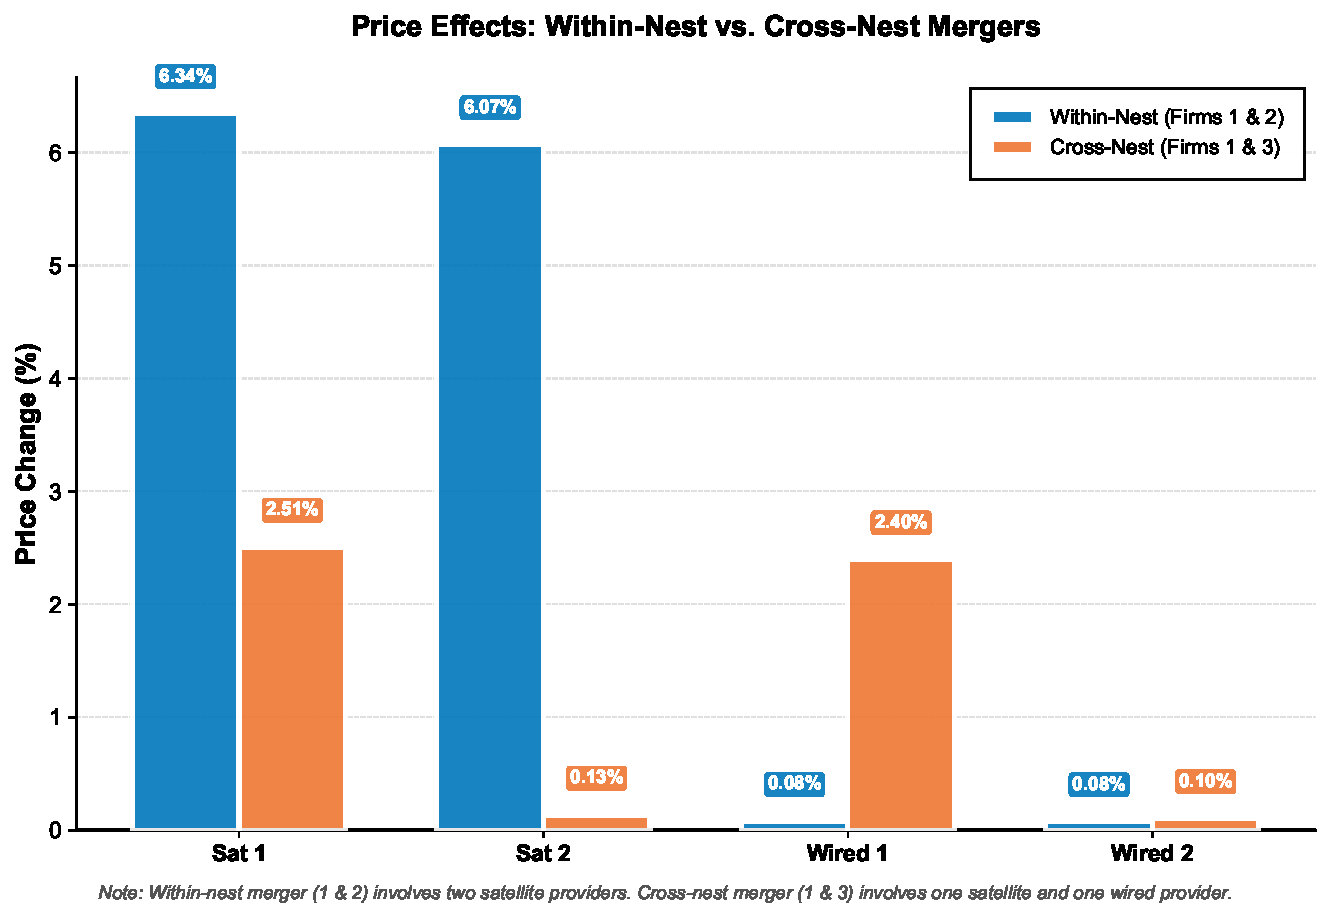
\includegraphics[width=0.85\textwidth]{merger_comparison.pdf}
\caption{Price Effects: Within-Nest vs. Cross-Nest Mergers. Grouped bars compare percentage price changes across all four products for two merger scenarios: within-nest merger of satellite providers (Firms 1 \& 2, blue) and cross-nest merger combining satellite and wired providers (Firms 1 \& 3, yellow). The within-nest merger produces substantially larger price increases for the merging satellite products (6.34\% and 6.07\%) compared to the cross-nest merger (2.51\% for Sat 1). This difference reflects higher diversion ratios within product categories: satellite consumers readily substitute between satellite options, creating stronger recapture incentives. The cross-nest merger generates modest price increases for both merging firms (2.51\% and 2.40\%) but minimal spillovers to non-merging products, demonstrating that substitution patterns between merging firms' products critically determine merger impacts.}
\label{fig:merger_comparison}
\end{figure}

The cross-nest merger of satellite provider (firm 1) and wired provider (firm 3) produces substantially smaller price increases than the within-nest merger. Merging firms 1 and 3 raise prices by approximately 2.5\% each, compared to 6\% increases when satellite competitors merged. This reflects lower diversion ratios between satellite and wired products: when firm 1 raises its satellite price, few consumers switch to firm 3's wired product, limiting the internalized externality. The within-nest merger internalizes higher diversion (satellite consumers readily substitute between satellite products), generating larger recapture effects and price increases. Non-merging firms show asymmetric responses: Sat 2 barely adjusts (0.13\%) when its competitor merges with a wired provider, while Wired 1 increases 2.40\% when satellite providers merge. This pattern confirms that competitive pressure operates primarily within product categories. The cross-nest merger reduces average prices (\$3.360 vs \$3.422) and increases consumer surplus (0.445 vs 0.432) relative to the within-nest merger, demonstrating that merger effects depend critically on substitution patterns between merging firms' products.

\item[14.] Thus far you have assumed that there are no \textquotedblleft
efficiencies\textquotedblright\ (reduction in costs) resulting from the
merger. Explain briefly why a merger-specific reduction in marginal cost
could mean that a merger is welfare-enhancing.

\textbf{Answer:}

Merger-specific marginal cost reductions create opposing welfare effects. The merger induces price increases through internalization of competitive externalities (unilateral effects), reducing consumer surplus. Simultaneously, lower marginal costs shift the pricing FOC, inducing price decreases. From the merged firm's FOC, $p_{jt} = mc_{jt} - (\partial s_{jt}/\partial p_{jt})^{-1} [s_{jt} + \sum_{k \in \mathcal{J}_{\text{merged}} \setminus \{j\}} (p_{kt} - mc_{kt}) \partial s_{kt}/\partial p_{jt}]$, a reduction in $mc_{jt}$ directly lowers optimal $p_{jt}$ even holding markup constant. The net price effect depends on which force dominates.

Consumer surplus may increase if cost reductions are large enough to offset unilateral effects, causing post-merger prices to fall. Even if prices rise modestly, partial pass-through of cost savings limits consumer harm. Producer surplus typically increases from both recaptured margins on diverted sales and lower production costs on all units sold, with cost savings accruing regardless of price changes. For total welfare, marginal cost reductions represent real resource savings---identical output produced with fewer inputs. This productive efficiency gain increases total surplus even if prices do not fall, as cost savings accrue to producers.

A merger enhances welfare when productive efficiency gains (cost savings times quantity) plus consumer surplus changes (from net price effects) exceed zero. Since consumer surplus changes depend on price changes, which depend on both cost reductions and diversion patterns, merger evaluation requires quantifying both effects through simulation. The efficiency must be merger-specific---achievable only through the merger, not via independent R\&D or contracts---to ensure the defense does not approve anti-competitive mergers claiming hypothetical savings. The welfare tradeoff between anti-competitive harm and efficiency gains is fundamentally quantitative.

\item[15.] Consider the merger between firms 1 and 2, and suppose the firms
demonstrate that by merging they would reduce marginal cost of each of their
products by 15\%. Furthermore, suppose that they demonstrate that this cost
reduction could not be achieved without merging.    Using the \texttt{pyBLP} software, re-run the merger simulation
with the 15\% cost saving. Show the predicted post-merger price changes (again,
for each product, averaged across markets). What is the predicted impact of
the merger on consumer welfare, assuming that the total measure of consumers $%
M_{t} $ is the same in each market  $t$?  

\begin{verbatim}
# Assume M_t = 1000 consumers per market (needed for welfare calculation)
M_t = 1000

# Get estimated marginal costs and apply 15% reduction to firms 1 and 2
marginal_costs = optimal_iv_results2.compute_costs()
marginal_costs_efficiency = marginal_costs.copy()
products_1_2 = product_data['firm_ids'].isin([1, 2])
marginal_costs_efficiency[products_1_2] *= 0.85

# Compute post-merger prices with efficiency gains
post_merger_prices_efficiency = optimal_iv_results2.compute_prices(
    firm_ids=merger_firm_ids,  # From Q12
    costs=marginal_costs_efficiency,
    iteration=pyblp.Iteration('simple', {'atol': 1e-12})
)

# Calculate price changes
post_merger_prices_eff_avg = post_merger_prices_efficiency.reshape((T, J)).mean(axis=0)
pct_price_changes_eff = ((post_merger_prices_eff_avg - pre_merger_prices_avg) 
                          / pre_merger_prices_avg) * 100

# Welfare analysis
cs_pre = optimal_iv_results2.compute_consumer_surpluses()
cs_post_no_eff = optimal_iv_results2.compute_consumer_surpluses(
    prices=post_merger_prices)
cs_post_with_eff = optimal_iv_results2.compute_consumer_surpluses(
    prices=post_merger_prices_efficiency)

# Total CS changes = M_t * sum over all markets
total_delta_cs_no_eff = M_t * (cs_post_no_eff - cs_pre).sum()
total_delta_cs_with_eff = M_t * (cs_post_with_eff - cs_pre).sum()

# Producer surplus: (p - mc) x shares x M_t
# Pre-merger, post-merger without efficiency, post-merger with efficiency
# Total welfare = DCS + DPS
\end{verbatim}

\textbf{Results:}

\textit{Price Changes with 15\% Cost Reduction:}

\begin{center}
\begin{tabular}{lcccccc}
\hline
Product & Firm (Pre) & Firm (Post) & Pre-Merger & Post-Merger & Change (\$) & Change (\%) \\
\hline
Sat 1 & 1 & 1 & 3.3381 & 3.2625 & $-0.0756$ & $-2.26$ \\
Sat 2 & 2 & 1 & 3.2858 & 3.2075 & $-0.0782$ & $-2.38$ \\
Wired 1 & 3 & 3 & 3.3210 & 3.3164 & $-0.0046$ & $-0.14$ \\
Wired 2 & 4 & 4 & 3.3253 & 3.3212 & $-0.0041$ & $-0.12$ \\
\hline
\end{tabular}
\end{center}

\textit{Comparison: No Efficiency vs 15\% Cost Reduction:}

\begin{center}
\begin{tabular}{lccc}
\hline
Product & No Efficiency (\%) & With 15\% Cost Cut (\%) & Difference (pp) \\
\hline
Sat 1 & 6.34 & $-2.26$ & $-8.61$ \\
Sat 2 & 6.07 & $-2.38$ & $-8.45$ \\
Wired 1 & 0.08 & $-0.14$ & $-0.22$ \\
Wired 2 & 0.08 & $-0.12$ & $-0.20$ \\
\hline
\end{tabular}
\end{center}

\textit{Welfare Analysis (assuming $M_t = 1{,}000$ consumers/market, $T = 600$ markets):}

\begin{center}
\begin{tabular}{lcccc}
\hline
Scenario & $\Delta$CS per capita (\$) & $\Delta$CS total (\$) & $\Delta$PS (\$) & $\Delta$W (\$) \\
\hline
Without efficiency & $-0.0301$ & $-18{,}043$ & $7{,}318$ & $-10{,}725$ \\
With 15\% cost cut & $0.0363$ & $21{,}805$ & $55{,}186$ & $76{,}990$ \\
\hline
\end{tabular}
\end{center}

\begin{figure}[h]
\centering
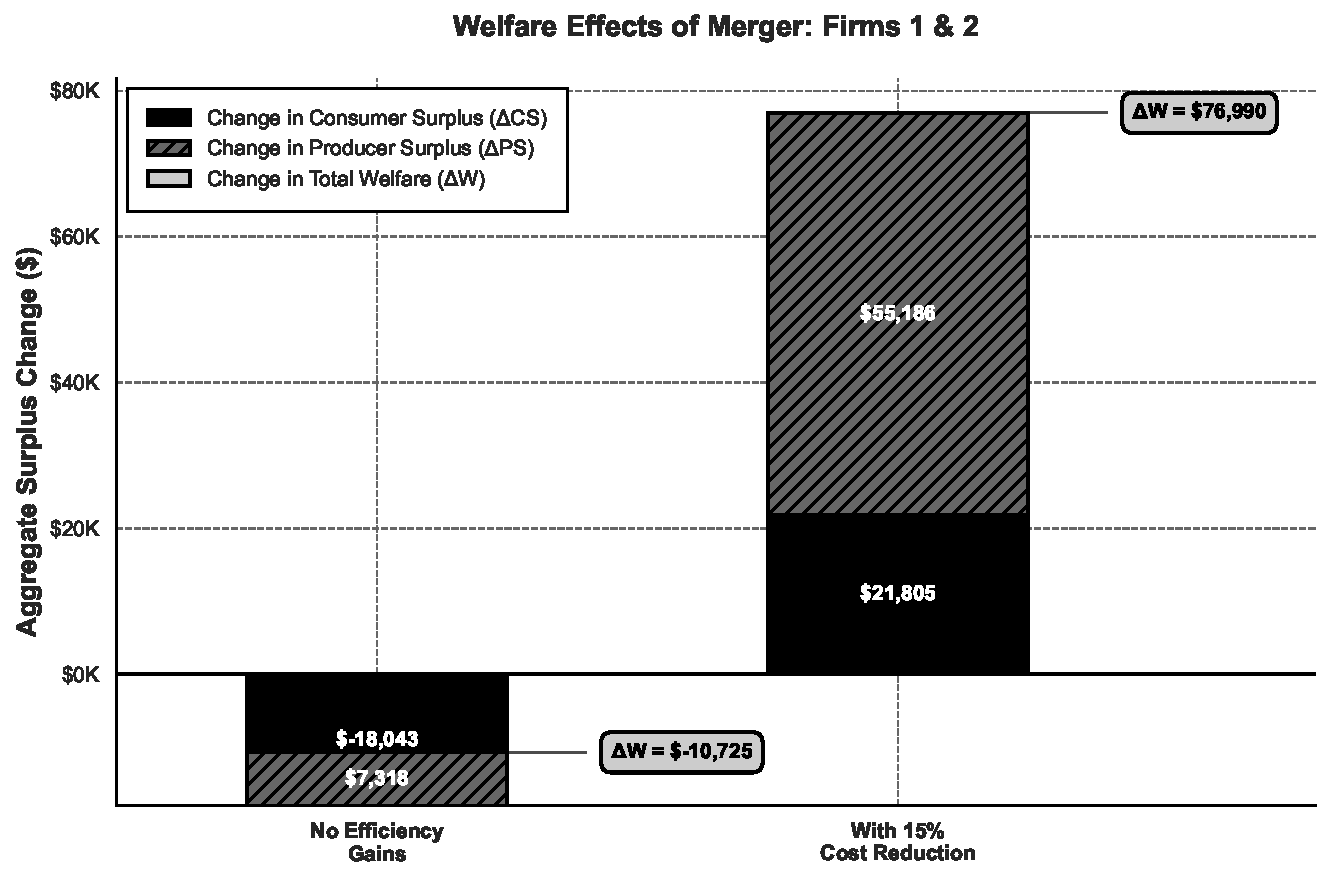
\includegraphics[width=0.85\textwidth]{surplus_changes_merger.pdf}
\caption{Welfare Effects of Satellite Merger (Firms 1 \& 2). Stacked bars show consumer surplus (blue) and producer surplus (orange) changes for two scenarios: merger without efficiency gains (left) and merger with 15\% cost reduction (right). Total welfare change ($\Delta W$) is shown above each bar. Without efficiency, the merger reduces total welfare by \$10,725 as consumer harm exceeds producer gain. With 15\% cost reduction, both consumer and producer surplus increase, yielding a total welfare gain of \$76,990. Values represent aggregate changes across all 600 markets with 1,000 consumers per market.}
\label{fig:surplus_changes}
\end{figure}

The 15\% cost reduction reverses merger price effects: merging satellite firms reduce prices by 2.3\% rather than increasing by 6\%. Non-merging wired firms respond with slight price decreases (0.13\%) as best responses. Without efficiency, the merger reduces total welfare by \$10,725 (consumer harm \$18,043 exceeds producer gain \$7,318). With efficiency, total welfare increases by \$76,990, decomposing into consumer surplus gain \$21,805 plus producer surplus gain \$55,186. Cost pass-through dominates unilateral effects: lower marginal costs shift pricing FOCs sufficiently to overcome recapture incentives, yielding price decreases. Producer surplus increases despite lower prices because cost savings (\$0.15 reduction $\times$ quantity sold) exceed markup erosion. The productive efficiency gain (real resource savings from lower costs) transforms a welfare-reducing merger into a welfare-enhancing one.

Explain why this additional assumption
(or data on the correct values of $M_{t}$) is needed here, whereas up to
this point it was without loss to assume $M_{t}=1$. What is the predicted
impact of the merger on total welfare?

\textbf{Answer:}

All prior analysis focused on per-capita quantities: market shares $s_{jt}$, prices $p_{jt}$, elasticities $\varepsilon_{jk}$, and diversion ratios $D_{jk}$. These are invariant to $M_t$ because they involve ratios of quantities or derivatives of shares. Market share $s_{jt} = Q_{jt}/M_t$ is a ratio, so normalizing $M_t = 1$ is without loss. Elasticity $\varepsilon_{jk} = (\partial s_j/\partial p_k) \cdot (p_k/s_j)$ involves derivatives of shares, independent of market size. Equilibrium prices satisfy $p_{jt} = mc_{jt} - (\partial s_{jt}/\partial p_{jt})^{-1} s_{jt}$, depending only on shares and their derivatives, not absolute quantities.

Consumer surplus, however, integrates willingness-to-pay across all consumers: $CS_t = M_t \cdot \int_i [u_i(\mathbf{p}^{\text{pre}}) - u_i(\mathbf{p}^{\text{post}})] dF(\text{type}_i)$. Using the logit compensating variation formula, $CS_t = M_t \cdot \mathbb{E}_{\beta_i, \epsilon_i} [(1/\alpha_i) (\ln \sum_j e^{\delta_j^{\text{pre}} + \nu_{ij}} - \ln \sum_j e^{\delta_j^{\text{post}} + \nu_{ij}})]$. Per-capita consumer surplus is invariant to $M_t$, but aggregate consumer surplus scales linearly with $M_t$. Without knowing $M_t$ or assuming constant $M_t$ across markets, we cannot compute total dollar value of consumer harm, weight welfare changes across markets of different sizes, or compare consumer surplus changes to producer surplus changes (which also scale with $M_t$).

Total welfare equals consumer surplus plus producer surplus. Producer surplus change from merger is $\Delta PS_t = M_t \sum_{j \in \mathcal{J}_{\text{merged}}} [(p_j^{\text{post}} - mc_j^{\text{post}}) s_j^{\text{post}} - (p_j^{\text{pre}} - mc_j^{\text{pre}}) s_j^{\text{pre}}] + M_t \sum_{j \notin \mathcal{J}_{\text{merged}}} [(p_j^{\text{post}} - mc_j^{\text{post}}) s_j^{\text{post}} - (p_j^{\text{pre}} - mc_j^{\text{pre}}) s_j^{\text{pre}}]$. With merger efficiencies ($mc_j^{\text{post}} < mc_j^{\text{pre}}$ for merged products), consumer surplus may increase or decrease depending on whether cost pass-through dominates unilateral price effects. Producer surplus typically increases from higher markups and cost savings on all units sold. Total welfare reflects productive efficiency gains (cost savings times quantity, representing real resource savings) minus deadweight loss from price changes reducing consumption.

The net welfare effect is $\Delta W_t = M_t \sum_j (mc_j^{\text{pre}} - mc_j^{\text{post}}) \cdot Q_j^{\text{post}} - M_t \cdot \text{DWL}$. If cost reductions are large (15\%), productive efficiency may dominate allocative inefficiency, yielding net welfare gains even if prices rise modestly. Prices and market structure can be analyzed with $M_t = 1$ (per-capita framework), but welfare statements require either data on actual $M_t$, assumption of constant $M_t$ for average per-capita welfare, or focus on percentage welfare changes (which are $M_t$-invariant).

\end{enumerate}

\subsection*{Summary: Consolidated Merger Diagnostics}

The table below consolidates key metrics across all merger scenarios analyzed:

\begin{center}
\small
\begin{tabular}{lccccccc}
\hline
Metric & Pre-Merger & \makecell{Merger 1\&2\\(No Eff)} & \makecell{Merger 1\&3\\(Cross)} & \makecell{Merger 1\&2\\(15\% Cut)} & \makecell{$\Delta$ (1\&2\\- Pre)} & \makecell{$\Delta$ (1\&3\\- Pre)} & \makecell{$\Delta$ (15\% Cut\\- Pre)} \\
\hline
Avg Price (\$) & 3.318 & 3.422 & 3.360 & 3.277 & 0.104 & 0.043 & $-0.041$ \\
Avg Markup (\$) & 0.204 & 0.227 & 0.214 & 0.254 & 0.023 & 0.010 & 0.050 \\
Total Profit (\$) & 268.51 & 275.82 & 272.24 & 323.69 & 7.32 & 3.73 & 55.19 \\
Avg CS (\$) & 0.462 & 0.432 & 0.445 & 0.498 & $-0.030$ & $-0.017$ & 0.036 \\
\hline
\end{tabular}
\end{center}

The within-nest merger without efficiencies (firms 1\&2) generates the largest price increase (\$0.104), while the cross-nest merger (firms 1\&3) produces moderate effects (\$0.043). The 15\% cost reduction reverses price effects entirely (\$$-$0.041 average price decrease). Average markups increase in all scenarios due to internalization of competitive externalities, with the largest markup increase (0.050) occurring under the efficiency scenario as cost reductions create room for higher percentage markups despite lower absolute prices. Total profit increases most with efficiency gains (\$55.19), combining cost savings with recaptured margins. Consumer surplus decreases under anti-competitive mergers ($-$0.030 for within-nest, $-$0.017 for cross-nest) but increases (0.036) when cost pass-through dominates unilateral effects. The cross-nest merger is less harmful than the within-nest merger across all metrics, confirming that substitution patterns between merging firms' products determine merger impacts.

\bibliographystyle{ecta}
\bibliography{BLP_hw_chadim}

\end{document}
